\chapter{Introduction}
\label{chapterlabel1}

Real-time Bidding (RTB) has become an important new paradigm in display advertising. It is a kind of online auction. eMarket estimates a 73$\%$ spending growth on RTB in US during 2013, which accounts for 19$\%$ of the total spending in display advertising \cite{emarketer2013}. The three major search engines Google, Yahoo and Bing generate revenue of at least 25 billion dollars per year from display advertising.

Supply-side platform (SSP) is created to serve publisher which can maximize the profit of publishers' impressions, such as OpenX, PubMatic, Rubicon Project and AppNexus. The idea of SSP is that publishers connect their inventory to multiple ad exchanges with some rules to find as many as potential buyers as possible through a real-time second price auction. 

Demand-side platform (DSP) is a third party platform where advertisers can purchase a variety of impressions based on identifying and creating different optimal bidding strategies. Many factors like impression features, budget and clickability will influence their bids for the campaign. The purpose of bidding strategies in DSP is to optimize advertisers' key performance indicator (KPI) for various clicks and conversions. According to Figure~\ref{fig:RTB} from \cite{Zhang:2014:ORB:2623330.2623633}, this figure gives a very clear and structural explanation of the whole process of RTB.

\begin{figure}[htbp]
\centering
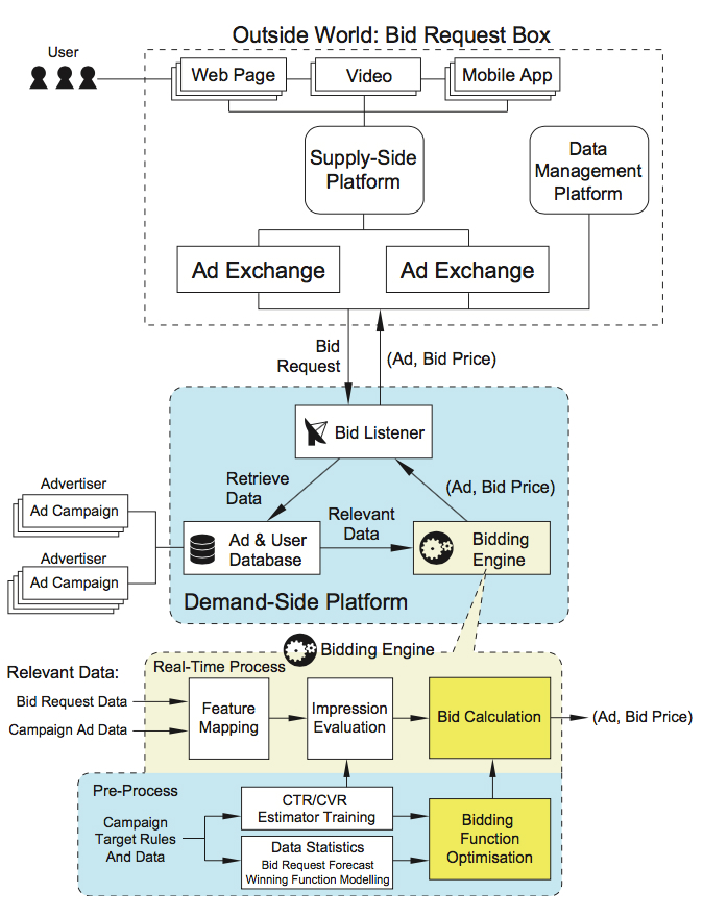
\includegraphics[width=0.70\textwidth]{RTB.pdf}
\caption{An illustration of a DSP and its bidding engine in RTB display advertising}
\label{fig:RTB}
\end{figure}

Certainly, there are interest conflicts between advertisers and publishers because the buy-side is KPI-oriented while the sell-side is revenue-oriented.

In RTB based display advertising, demand side platforms (DSPs) usually estimate the Click-through Rate (CTR) of each impression and then decide whether and how much to bid based on the behaviour of advertisers.

In online auctions, new ads that may compete in the auctions are constantly entering the system, and for these ads, one will have uncertainty for market price landscape because of the fact that one will not know the CTR of a new ad. Thus, advertisers need to explore the preference of the market and also discover the CTR of this impression after winning it.

We research on an application of combination of auction and CTR estimation, which forms the repeated auction. In this project, we mainly focus on the following two cases:

\begin{enumerate}

\item A simplest situation is for one-shot RTB auction and each advertiser knows their own CTR. We want to find out the optimal bid price for advertisers.

\item A slightly more complicated case is that the auction repeated running finitely. In this case, each advertiser still knows their own CTR. What is the optimal bidding strategy? Are we getting the same result as in the previous case or something different? In this case, as each advertiser knows their value so no information exploration for true value, but they can have an exploration on the market price landscape. Intuitively, we should get a higher bid than the previous case or we would obtain the same conclusion.

\end{enumerate}
The structure of the thesis is shown below:
\begin{itemize}

 \item Chapter 2: \emph{Click-through Rate (CTR) Prediction} \\
This chapter provides a concise review of the advanced and practical CTR prediction models. The introduction starts from Bayesian Online Probit Regression (BOPR), Follow the Regularized Leader (FTRL) and Field-aware Factorization Machine (FFM). Also, the dataset that we use is described in this chapter, followed by some preprocessing and feature engineering techniques.

\item Chapter 3: \emph{Auction Theory} \\
In this chapter, we discuss the typical auction theory which is used in online advertising. The most commonly applied auction is sealed first-price bid and sealed second-price bid. RTB, Sponsored Search and some other ranking mechanisms follow the similar ways. According to the closed form solutions of these two kinds of auction as games, there are two conclusions to the bidding price based on the true value. 

\item Chapter 4: \emph{Active Learning in Real-time Bidding (RTB)} \\
When it refers to RTB, \emph{exploition-exploration} always happens since no advertiser knows the information from the market at the first time. For the purpose of maximising present utility, they may bid a price to test the market and actively learn from the feedbacks. This sacrifice may increase the utility in the future. In this chapter, we consider two cases. They are one-shot auction and finite sequential auctions respectively.

\item Chapter 5: \emph{Summary and Discussion of Results} \\
This chapter mainly focuses on the implementation part of the project. We will give the experimental results and compare different methods. The discussion covers the advantage and disadvantage of all techniques. Also, after this procedure, we do some simulations on the RTB problems. 

\item Chapter 6: \emph{Conclusions and Future Work} \\
The final chapter presents the conclusions of the theoretical and experimental studies implemented throughout the project. The achievement and a brief summary is included in this section.The general guidance for further potential research are finally discussed.

\end{itemize}

